\documentclass[1p]{elsarticle_modified}
%\bibliographystyle{elsarticle-num}

%\usepackage[colorlinks]{hyperref}
%\usepackage{abbrmath_seonhwa} %\Abb, \Ascr, \Acal ,\Abf, \Afrak
\usepackage{amsfonts}
\usepackage{amssymb}
\usepackage{amsmath}
\usepackage{amsthm}
\usepackage{scalefnt}
\usepackage{amsbsy}
\usepackage{kotex}
\usepackage{caption}
\usepackage{subfig}
\usepackage{color}
\usepackage{graphicx}
\usepackage{xcolor} %% white, black, red, green, blue, cyan, magenta, yellow
\usepackage{float}
\usepackage{setspace}
\usepackage{hyperref}

\usepackage{tikz}
\usetikzlibrary{arrows}

\usepackage{multirow}
\usepackage{array} % fixed length table
\usepackage{hhline}

%%%%%%%%%%%%%%%%%%%%%
\makeatletter
\renewcommand*\env@matrix[1][\arraystretch]{%
	\edef\arraystretch{#1}%
	\hskip -\arraycolsep
	\let\@ifnextchar\new@ifnextchar
	\array{*\c@MaxMatrixCols c}}
\makeatother %https://tex.stackexchange.com/questions/14071/how-can-i-increase-the-line-spacing-in-a-matrix
%%%%%%%%%%%%%%%

\usepackage[normalem]{ulem}

\newcommand{\msout}[1]{\ifmmode\text{\sout{\ensuremath{#1}}}\else\sout{#1}\fi}
%SOURCE: \msout is \stkout macro in https://tex.stackexchange.com/questions/20609/strikeout-in-math-mode

\newcommand{\cancel}[1]{
	\ifmmode
	{\color{red}\msout{#1}}
	\else
	{\color{red}\sout{#1}}
	\fi
}

\newcommand{\add}[1]{
	{\color{blue}\uwave{#1}}
}

\newcommand{\replace}[2]{
	\ifmmode
	{\color{red}\msout{#1}}{\color{blue}\uwave{#2}}
	\else
	{\color{red}\sout{#1}}{\color{blue}\uwave{#2}}
	\fi
}

\newcommand{\Sol}{\mathcal{S}} %segment
\newcommand{\D}{D} %diagram
\newcommand{\A}{\mathcal{A}} %arc


%%%%%%%%%%%%%%%%%%%%%%%%%%%%%5 test

\def\sl{\operatorname{\textup{SL}}(2,\Cbb)}
\def\psl{\operatorname{\textup{PSL}}(2,\Cbb)}
\def\quan{\mkern 1mu \triangleright \mkern 1mu}

\theoremstyle{definition}
\newtheorem{thm}{Theorem}[section]
\newtheorem{prop}[thm]{Proposition}
\newtheorem{lem}[thm]{Lemma}
\newtheorem{ques}[thm]{Question}
\newtheorem{cor}[thm]{Corollary}
\newtheorem{defn}[thm]{Definition}
\newtheorem{exam}[thm]{Example}
\newtheorem{rmk}[thm]{Remark}
\newtheorem{alg}[thm]{Algorithm}

\newcommand{\I}{\sqrt{-1}}
\begin{document}

%\begin{frontmatter}
%
%\title{Boundary parabolic representations of knots up to 8 crossings}
%
%%% Group authors per affiliation:
%\author{Yunhi Cho} 
%\address{Department of Mathematics, University of Seoul, Seoul, Korea}
%\ead{yhcho@uos.ac.kr}
%
%
%\author{Seonhwa Kim} %\fnref{s_kim}}
%\address{Center for Geometry and Physics, Institute for Basic Science, Pohang, 37673, Korea}
%\ead{ryeona17@ibs.re.kr}
%
%\author{Hyuk Kim}
%\address{Department of Mathematical Sciences, Seoul National University, Seoul 08826, Korea}
%\ead{hyukkim@snu.ac.kr}
%
%\author{Seokbeom Yoon}
%\address{Department of Mathematical Sciences, Seoul National University, Seoul, 08826,  Korea}
%\ead{sbyoon15@snu.ac.kr}
%
%\begin{abstract}
%We find all boundary parabolic representation of knots up to 8 crossings.
%
%\end{abstract}
%\begin{keyword}
%    \MSC[2010] 57M25 
%\end{keyword}
%
%\end{frontmatter}

%\linenumbers
%\tableofcontents
%
\newcommand\colored[1]{\textcolor{white}{\rule[-0.35ex]{0.8em}{1.4ex}}\kern-0.8em\color{red} #1}%
%\newcommand\colored[1]{\textcolor{white}{ #1}\kern-2.17ex	\textcolor{white}{ #1}\kern-1.81ex	\textcolor{white}{ #1}\kern-2.15ex\color{red}#1	}

{\Large $\underline{12a_{0674}~(K12a_{0674})}$}

\setlength{\tabcolsep}{10pt}
\renewcommand{\arraystretch}{1.6}
\vspace{1cm}\begin{tabular}{m{100pt}>{\centering\arraybackslash}m{274pt}}
\multirow{5}{120pt}{
	\centering
	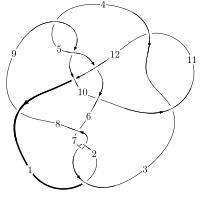
\includegraphics[width=112pt]{../../../GIT/diagram.site/Diagrams/png/1475_12a_0674.png}\\
\ \ \ A knot diagram\footnotemark}&
\allowdisplaybreaks
\textbf{Linearized knot diagam} \\
\cline{2-2}
 &
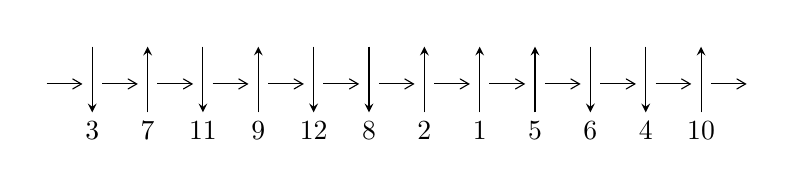
\begin{tikzpicture}[x=20pt, y=17pt]
	% nodes
	\node (C0) at (0, 0) {};
	\node (C1) at (1, 0) {};
	\node (C1U) at (1, +1) {};
	\node (C1D) at (1, -1) {3};

	\node (C2) at (2, 0) {};
	\node (C2U) at (2, +1) {};
	\node (C2D) at (2, -1) {7};

	\node (C3) at (3, 0) {};
	\node (C3U) at (3, +1) {};
	\node (C3D) at (3, -1) {11};

	\node (C4) at (4, 0) {};
	\node (C4U) at (4, +1) {};
	\node (C4D) at (4, -1) {9};

	\node (C5) at (5, 0) {};
	\node (C5U) at (5, +1) {};
	\node (C5D) at (5, -1) {12};

	\node (C6) at (6, 0) {};
	\node (C6U) at (6, +1) {};
	\node (C6D) at (6, -1) {8};

	\node (C7) at (7, 0) {};
	\node (C7U) at (7, +1) {};
	\node (C7D) at (7, -1) {2};

	\node (C8) at (8, 0) {};
	\node (C8U) at (8, +1) {};
	\node (C8D) at (8, -1) {1};

	\node (C9) at (9, 0) {};
	\node (C9U) at (9, +1) {};
	\node (C9D) at (9, -1) {5};

	\node (C10) at (10, 0) {};
	\node (C10U) at (10, +1) {};
	\node (C10D) at (10, -1) {6};

	\node (C11) at (11, 0) {};
	\node (C11U) at (11, +1) {};
	\node (C11D) at (11, -1) {4};

	\node (C12) at (12, 0) {};
	\node (C12U) at (12, +1) {};
	\node (C12D) at (12, -1) {10};
	\node (C13) at (13, 0) {};

	% arrows
	\draw[->,>={angle 60}]
	(C0) edge (C1) (C1) edge (C2) (C2) edge (C3) (C3) edge (C4) (C4) edge (C5) (C5) edge (C6) (C6) edge (C7) (C7) edge (C8) (C8) edge (C9) (C9) edge (C10) (C10) edge (C11) (C11) edge (C12) (C12) edge (C13) ;	\draw[->,>=stealth]
	(C1U) edge (C1D) (C2D) edge (C2U) (C3U) edge (C3D) (C4D) edge (C4U) (C5U) edge (C5D) (C6U) edge (C6D) (C7D) edge (C7U) (C8D) edge (C8U) (C9D) edge (C9U) (C10U) edge (C10D) (C11U) edge (C11D) (C12D) edge (C12U) ;
	\end{tikzpicture} \\
\hhline{~~} \\& 
\textbf{Solving Sequence} \\ \cline{2-2} 
 &
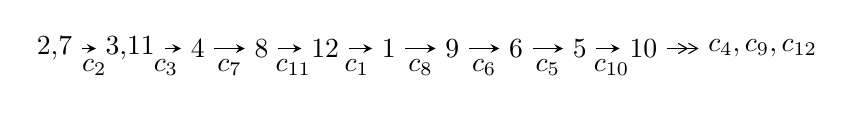
\begin{tikzpicture}[x=23pt, y=7pt]
	% node
	\node (A0) at (-1/8, 0) {2,7};
	\node (A1) at (17/16, 0) {3,11};
	\node (A2) at (17/8, 0) {4};
	\node (A3) at (25/8, 0) {8};
	\node (A4) at (33/8, 0) {12};
	\node (A5) at (41/8, 0) {1};
	\node (A6) at (49/8, 0) {9};
	\node (A7) at (57/8, 0) {6};
	\node (A8) at (65/8, 0) {5};
	\node (A9) at (73/8, 0) {10};
	\node (C1) at (1/2, -1) {$c_{2}$};
	\node (C2) at (13/8, -1) {$c_{3}$};
	\node (C3) at (21/8, -1) {$c_{7}$};
	\node (C4) at (29/8, -1) {$c_{11}$};
	\node (C5) at (37/8, -1) {$c_{1}$};
	\node (C6) at (45/8, -1) {$c_{8}$};
	\node (C7) at (53/8, -1) {$c_{6}$};
	\node (C8) at (61/8, -1) {$c_{5}$};
	\node (C9) at (69/8, -1) {$c_{10}$};
	\node (A10) at (11, 0) {$c_{4},c_{9},c_{12}$};

	% edge
	\draw[->,>=stealth]	
	(A0) edge (A1) (A1) edge (A2) (A2) edge (A3) (A3) edge (A4) (A4) edge (A5) (A5) edge (A6) (A6) edge (A7) (A7) edge (A8) (A8) edge (A9) ;
	\draw[->>,>={angle 60}]	
	(A9) edge (A10);
\end{tikzpicture} \\ 

\end{tabular} \\

\footnotetext{
The image of knot diagram is generated by the software ``\textbf{Draw programme}" developed by Andrew Bartholomew(\url{http://www.layer8.co.uk/maths/draw/index.htm\#Running-draw}), where we modified some parts for our purpose(\url{https://github.com/CATsTAILs/LinksPainter}).
}\phantom \\ \newline 
\centering \textbf{Ideals for irreducible components\footnotemark of $X_{\text{par}}$} 
 
\begin{align*}
I^u_{1}&=\langle 
7.30354\times10^{106} u^{132}+1.06306\times10^{107} u^{131}+\cdots+2.46021\times10^{107} b+6.28959\times10^{107},\\
\phantom{I^u_{1}}&\phantom{= \langle  }-1.10982\times10^{109} u^{132}+1.75925\times10^{109} u^{131}+\cdots+1.30391\times10^{109} a+6.69976\times10^{107},\\
\phantom{I^u_{1}}&\phantom{= \langle  }u^{133}- u^{132}+\cdots+11 u-1\rangle \\
I^u_{2}&=\langle 
- u^{22}-2 u^{20}+\cdots+b+1,\;u^{22}+5 u^{20}+\cdots+a-3,\;u^{23}+4 u^{21}+\cdots-4 u^2-1\rangle \\
\\
\end{align*}
\raggedright * 2 irreducible components of $\dim_{\mathbb{C}}=0$, with total 156 representations.\\
\footnotetext{All coefficients of polynomials are rational numbers. But the coefficients are sometimes approximated in decimal forms when there is not enough margin.}
\newpage
\renewcommand{\arraystretch}{1}
\centering \section*{I. $I^u_{1}= \langle 7.30\times10^{106} u^{132}+1.06\times10^{107} u^{131}+\cdots+2.46\times10^{107} b+6.29\times10^{107},\;-1.11\times10^{109} u^{132}+1.76\times10^{109} u^{131}+\cdots+1.30\times10^{109} a+6.70\times10^{107},\;u^{133}- u^{132}+\cdots+11 u-1 \rangle$}
\flushleft \textbf{(i) Arc colorings}\\
\begin{tabular}{m{7pt} m{180pt} m{7pt} m{180pt} }
\flushright $a_{2}=$&$\begin{pmatrix}1\\0\end{pmatrix}$ \\
\flushright $a_{7}=$&$\begin{pmatrix}0\\u\end{pmatrix}$ \\
\flushright $a_{3}=$&$\begin{pmatrix}1\\- u^2\end{pmatrix}$ \\
\flushright $a_{11}=$&$\begin{pmatrix}0.851148 u^{132}-1.34921 u^{131}+\cdots-26.4094 u-0.0513820\\-0.296866 u^{132}-0.432100 u^{131}+\cdots+15.0390 u-2.55652\end{pmatrix}$ \\
\flushright $a_{4}=$&$\begin{pmatrix}3.22970 u^{132}-2.96146 u^{131}+\cdots-120.446 u+17.4193\\-0.418462 u^{132}-0.951295 u^{131}+\cdots-20.2704 u+3.94279\end{pmatrix}$ \\
\flushright $a_{8}=$&$\begin{pmatrix}u\\u\end{pmatrix}$ \\
\flushright $a_{12}=$&$\begin{pmatrix}3.63001 u^{132}-2.81263 u^{131}+\cdots-119.194 u+18.3141\\0.283591 u^{132}+0.101456 u^{131}+\cdots-4.05479 u+1.29525\end{pmatrix}$ \\
\flushright $a_{1}=$&$\begin{pmatrix}u^2+1\\- u^4\end{pmatrix}$ \\
\flushright $a_{9}=$&$\begin{pmatrix}u^7+2 u^5+2 u^3+2 u\\- u^9- u^7- u^5+u\end{pmatrix}$ \\
\flushright $a_{6}=$&$\begin{pmatrix}u^3\\u^3+u\end{pmatrix}$ \\
\flushright $a_{5}=$&$\begin{pmatrix}2.16708 u^{132}-2.13527 u^{131}+\cdots-100.925 u+14.9635\\-1.70344 u^{132}-0.445984 u^{131}+\cdots-7.88626 u+2.51137\end{pmatrix}$ \\
\flushright $a_{10}=$&$\begin{pmatrix}1.14813 u^{132}-0.647471 u^{131}+\cdots-25.9002 u-0.124938\\-0.299784 u^{132}+0.495982 u^{131}+\cdots+22.2916 u-3.35175\end{pmatrix}$\\&\end{tabular}
\flushleft \textbf{(ii) Obstruction class $= -1$}\\~\\
\flushleft \textbf{(iii) Cusp Shapes $= -4.84648 u^{132}+2.26486 u^{131}+\cdots+85.5361 u-9.94143$}\\~\\
\newpage\renewcommand{\arraystretch}{1}
\flushleft \textbf{(iv) u-Polynomials at the component}\newline \\
\begin{tabular}{m{50pt}|m{274pt}}
Crossings & \hspace{64pt}u-Polynomials at each crossing \\
\hline $$\begin{aligned}c_{1},c_{6}\end{aligned}$$&$\begin{aligned}
&u^{133}+45 u^{132}+\cdots+21 u-1
\end{aligned}$\\
\hline $$\begin{aligned}c_{2},c_{7}\end{aligned}$$&$\begin{aligned}
&u^{133}+u^{132}+\cdots+11 u+1
\end{aligned}$\\
\hline $$\begin{aligned}c_{3},c_{11}\end{aligned}$$&$\begin{aligned}
&u^{133}-47 u^{131}+\cdots+8432 u+2069
\end{aligned}$\\
\hline $$\begin{aligned}c_{4},c_{9}\end{aligned}$$&$\begin{aligned}
&u^{133}-40 u^{131}+\cdots-1016 u-121
\end{aligned}$\\
\hline $$\begin{aligned}c_{5}\end{aligned}$$&$\begin{aligned}
&u^{133}- u^{132}+\cdots+17 u+3
\end{aligned}$\\
\hline $$\begin{aligned}c_{8}\end{aligned}$$&$\begin{aligned}
&u^{133}-5 u^{132}+\cdots+5531185 u+580413
\end{aligned}$\\
\hline $$\begin{aligned}c_{10}\end{aligned}$$&$\begin{aligned}
&u^{133}+3 u^{132}+\cdots-154743 u-114143
\end{aligned}$\\
\hline $$\begin{aligned}c_{12}\end{aligned}$$&$\begin{aligned}
&u^{133}+19 u^{132}+\cdots+419 u-11
\end{aligned}$\\
\hline
\end{tabular}\\~\\
\newpage\renewcommand{\arraystretch}{1}
\flushleft \textbf{(v) Riley Polynomials at the component}\newline \\
\begin{tabular}{m{50pt}|m{274pt}}
Crossings & \hspace{64pt}Riley Polynomials at each crossing \\
\hline $$\begin{aligned}c_{1},c_{6}\end{aligned}$$&$\begin{aligned}
&y^{133}+89 y^{132}+\cdots+225 y-1
\end{aligned}$\\
\hline $$\begin{aligned}c_{2},c_{7}\end{aligned}$$&$\begin{aligned}
&y^{133}+45 y^{132}+\cdots+21 y-1
\end{aligned}$\\
\hline $$\begin{aligned}c_{3},c_{11}\end{aligned}$$&$\begin{aligned}
&y^{133}-94 y^{132}+\cdots+138510782 y-4280761
\end{aligned}$\\
\hline $$\begin{aligned}c_{4},c_{9}\end{aligned}$$&$\begin{aligned}
&y^{133}-80 y^{132}+\cdots+653284 y-14641
\end{aligned}$\\
\hline $$\begin{aligned}c_{5}\end{aligned}$$&$\begin{aligned}
&y^{133}+5 y^{132}+\cdots+175 y-9
\end{aligned}$\\
\hline $$\begin{aligned}c_{8}\end{aligned}$$&$\begin{aligned}
&y^{133}+49 y^{132}+\cdots+385483097599 y-336879250569
\end{aligned}$\\
\hline $$\begin{aligned}c_{10}\end{aligned}$$&$\begin{aligned}
&y^{133}-25 y^{132}+\cdots+297383627417 y-13028624449
\end{aligned}$\\
\hline $$\begin{aligned}c_{12}\end{aligned}$$&$\begin{aligned}
&y^{133}-19 y^{132}+\cdots+229791 y-121
\end{aligned}$\\
\hline
\end{tabular}\\~\\
\newpage\flushleft \textbf{(vi) Complex Volumes and Cusp Shapes}
$$\begin{array}{c|c|c}  
\text{Solutions to }I^u_{1}& \I (\text{vol} + \sqrt{-1}CS) & \text{Cusp shape}\\
 \hline 
\begin{aligned}
u &= \phantom{-}0.829466 + 0.557218 I \\
a &= -0.187671 - 0.453469 I \\
b &= -1.222830 + 0.285357 I\end{aligned}
 & \phantom{-}0.27659 - 1.61748 I & \phantom{-0.000000 } 0 \\ \hline\begin{aligned}
u &= \phantom{-}0.829466 - 0.557218 I \\
a &= -0.187671 + 0.453469 I \\
b &= -1.222830 - 0.285357 I\end{aligned}
 & \phantom{-}0.27659 + 1.61748 I & \phantom{-0.000000 } 0 \\ \hline\begin{aligned}
u &= -0.734358 + 0.685968 I \\
a &= -0.716811 - 0.659771 I \\
b &= \phantom{-}1.83044 - 0.96506 I\end{aligned}
 & \phantom{-}3.13923 + 3.76117 I & \phantom{-0.000000 } 0 \\ \hline\begin{aligned}
u &= -0.734358 - 0.685968 I \\
a &= -0.716811 + 0.659771 I \\
b &= \phantom{-}1.83044 + 0.96506 I\end{aligned}
 & \phantom{-}3.13923 - 3.76117 I & \phantom{-0.000000 } 0 \\ \hline\begin{aligned}
u &= -0.721478 + 0.676585 I \\
a &= -1.15819 + 1.11373 I \\
b &= -2.41017 - 0.73023 I\end{aligned}
 & -1.030550 + 0.687025 I & \phantom{-0.000000 } 0 \\ \hline\begin{aligned}
u &= -0.721478 - 0.676585 I \\
a &= -1.15819 - 1.11373 I \\
b &= -2.41017 + 0.73023 I\end{aligned}
 & -1.030550 - 0.687025 I & \phantom{-0.000000 } 0 \\ \hline\begin{aligned}
u &= \phantom{-}0.031969 + 1.014520 I \\
a &= \phantom{-}2.90854 - 0.41681 I \\
b &= \phantom{-}1.91497 - 0.49345 I\end{aligned}
 & -2.20674 + 3.68448 I & \phantom{-0.000000 } 0 \\ \hline\begin{aligned}
u &= \phantom{-}0.031969 - 1.014520 I \\
a &= \phantom{-}2.90854 + 0.41681 I \\
b &= \phantom{-}1.91497 + 0.49345 I\end{aligned}
 & -2.20674 - 3.68448 I & \phantom{-0.000000 } 0 \\ \hline\begin{aligned}
u &= \phantom{-}0.016803 + 1.017960 I \\
a &= -2.03758 - 0.46975 I \\
b &= -0.510962 - 0.798251 I\end{aligned}
 & -6.25026 + 0.49451 I & \phantom{-0.000000 } 0 \\ \hline\begin{aligned}
u &= \phantom{-}0.016803 - 1.017960 I \\
a &= -2.03758 + 0.46975 I \\
b &= -0.510962 + 0.798251 I\end{aligned}
 & -6.25026 - 0.49451 I & \phantom{-0.000000 } 0\\
 \hline 
 \end{array}$$\newpage$$\begin{array}{c|c|c}  
\text{Solutions to }I^u_{1}& \I (\text{vol} + \sqrt{-1}CS) & \text{Cusp shape}\\
 \hline 
\begin{aligned}
u &= \phantom{-}0.685834 + 0.699198 I \\
a &= -0.767536 + 0.775321 I \\
b &= -1.028360 + 0.947545 I\end{aligned}
 & -1.47271 + 0.24934 I & \phantom{-0.000000 } 0 \\ \hline\begin{aligned}
u &= \phantom{-}0.685834 - 0.699198 I \\
a &= -0.767536 - 0.775321 I \\
b &= -1.028360 - 0.947545 I\end{aligned}
 & -1.47271 - 0.24934 I & \phantom{-0.000000 } 0 \\ \hline\begin{aligned}
u &= \phantom{-}0.727677 + 0.651708 I \\
a &= \phantom{-}0.35106 - 1.47593 I \\
b &= -1.36670 - 0.80541 I\end{aligned}
 & \phantom{-}1.24829 - 2.40392 I & \phantom{-0.000000 } 0 \\ \hline\begin{aligned}
u &= \phantom{-}0.727677 - 0.651708 I \\
a &= \phantom{-}0.35106 + 1.47593 I \\
b &= -1.36670 + 0.80541 I\end{aligned}
 & \phantom{-}1.24829 + 2.40392 I & \phantom{-0.000000 } 0 \\ \hline\begin{aligned}
u &= -0.179511 + 0.956362 I \\
a &= -0.351454 - 0.626307 I \\
b &= -0.635097 - 0.599965 I\end{aligned}
 & -0.91600 - 2.47222 I & \phantom{-0.000000 } 0 \\ \hline\begin{aligned}
u &= -0.179511 - 0.956362 I \\
a &= -0.351454 + 0.626307 I \\
b &= -0.635097 + 0.599965 I\end{aligned}
 & -0.91600 + 2.47222 I & \phantom{-0.000000 } 0 \\ \hline\begin{aligned}
u &= \phantom{-}0.660567 + 0.714040 I \\
a &= -0.58202 + 1.66891 I \\
b &= \phantom{-}2.34706 + 0.70544 I\end{aligned}
 & \phantom{-}2.31625 + 3.39587 I & \phantom{-0.000000 } 0 \\ \hline\begin{aligned}
u &= \phantom{-}0.660567 - 0.714040 I \\
a &= -0.58202 - 1.66891 I \\
b &= \phantom{-}2.34706 - 0.70544 I\end{aligned}
 & \phantom{-}2.31625 - 3.39587 I & \phantom{-0.000000 } 0 \\ \hline\begin{aligned}
u &= \phantom{-}0.620877 + 0.821547 I \\
a &= -0.48379 + 2.02623 I \\
b &= \phantom{-}1.33843 + 2.03608 I\end{aligned}
 & \phantom{-}2.29662 + 5.56622 I & \phantom{-0.000000 } 0 \\ \hline\begin{aligned}
u &= \phantom{-}0.620877 - 0.821547 I \\
a &= -0.48379 - 2.02623 I \\
b &= \phantom{-}1.33843 - 2.03608 I\end{aligned}
 & \phantom{-}2.29662 - 5.56622 I & \phantom{-0.000000 } 0\\
 \hline 
 \end{array}$$\newpage$$\begin{array}{c|c|c}  
\text{Solutions to }I^u_{1}& \I (\text{vol} + \sqrt{-1}CS) & \text{Cusp shape}\\
 \hline 
\begin{aligned}
u &= \phantom{-}0.748353 + 0.607521 I \\
a &= -0.64066 - 1.32225 I \\
b &= -2.30820 - 0.01910 I\end{aligned}
 & -0.55990 - 4.34234 I & \phantom{-0.000000 } 0 \\ \hline\begin{aligned}
u &= \phantom{-}0.748353 - 0.607521 I \\
a &= -0.64066 + 1.32225 I \\
b &= -2.30820 + 0.01910 I\end{aligned}
 & -0.55990 + 4.34234 I & \phantom{-0.000000 } 0 \\ \hline\begin{aligned}
u &= -0.806815 + 0.650210 I \\
a &= \phantom{-}0.78857 - 1.39267 I \\
b &= \phantom{-}2.49807 + 0.68797 I\end{aligned}
 & -2.09601 + 6.69318 I & \phantom{-0.000000 } 0 \\ \hline\begin{aligned}
u &= -0.806815 - 0.650210 I \\
a &= \phantom{-}0.78857 + 1.39267 I \\
b &= \phantom{-}2.49807 - 0.68797 I\end{aligned}
 & -2.09601 - 6.69318 I & \phantom{-0.000000 } 0 \\ \hline\begin{aligned}
u &= -0.792322 + 0.671448 I \\
a &= -0.02810 + 1.77382 I \\
b &= -1.74411 + 0.97162 I\end{aligned}
 & \phantom{-}5.33307 + 6.48914 I & \phantom{-0.000000 } 0 \\ \hline\begin{aligned}
u &= -0.792322 - 0.671448 I \\
a &= -0.02810 - 1.77382 I \\
b &= -1.74411 - 0.97162 I\end{aligned}
 & \phantom{-}5.33307 - 6.48914 I & \phantom{-0.000000 } 0 \\ \hline\begin{aligned}
u &= -0.032707 + 1.038950 I \\
a &= -0.471645 + 0.065998 I \\
b &= -0.405838 + 0.767883 I\end{aligned}
 & -4.17499 - 2.01012 I & \phantom{-0.000000 } 0 \\ \hline\begin{aligned}
u &= -0.032707 - 1.038950 I \\
a &= -0.471645 - 0.065998 I \\
b &= -0.405838 - 0.767883 I\end{aligned}
 & -4.17499 + 2.01012 I & \phantom{-0.000000 } 0 \\ \hline\begin{aligned}
u &= -0.715840 + 0.754563 I \\
a &= \phantom{-}0.31363 + 2.33969 I \\
b &= -1.53396 + 1.06766 I\end{aligned}
 & \phantom{-}4.04153 - 3.28866 I & \phantom{-0.000000 } 0 \\ \hline\begin{aligned}
u &= -0.715840 - 0.754563 I \\
a &= \phantom{-}0.31363 - 2.33969 I \\
b &= -1.53396 - 1.06766 I\end{aligned}
 & \phantom{-}4.04153 + 3.28866 I & \phantom{-0.000000 } 0\\
 \hline 
 \end{array}$$\newpage$$\begin{array}{c|c|c}  
\text{Solutions to }I^u_{1}& \I (\text{vol} + \sqrt{-1}CS) & \text{Cusp shape}\\
 \hline 
\begin{aligned}
u &= \phantom{-}0.098442 + 1.043060 I \\
a &= -0.279989 + 0.448295 I \\
b &= -0.167892 - 0.716442 I\end{aligned}
 & -0.76631 + 6.36624 I & \phantom{-0.000000 } 0 \\ \hline\begin{aligned}
u &= \phantom{-}0.098442 - 1.043060 I \\
a &= -0.279989 - 0.448295 I \\
b &= -0.167892 + 0.716442 I\end{aligned}
 & -0.76631 - 6.36624 I & \phantom{-0.000000 } 0 \\ \hline\begin{aligned}
u &= -0.616430 + 0.717140 I \\
a &= -0.031952 - 0.983535 I \\
b &= \phantom{-}0.457556 - 0.705776 I\end{aligned}
 & \phantom{-}0.299724 - 1.340940 I & \phantom{-0.000000 } 0 \\ \hline\begin{aligned}
u &= -0.616430 - 0.717140 I \\
a &= -0.031952 + 0.983535 I \\
b &= \phantom{-}0.457556 + 0.705776 I\end{aligned}
 & \phantom{-}0.299724 + 1.340940 I & \phantom{-0.000000 } 0 \\ \hline\begin{aligned}
u &= \phantom{-}0.843693 + 0.642382 I \\
a &= \phantom{-}0.80794 + 1.17541 I \\
b &= \phantom{-}2.40663 - 0.59239 I\end{aligned}
 & \phantom{-}1.37915 - 13.20260 I & \phantom{-0.000000 } 0 \\ \hline\begin{aligned}
u &= \phantom{-}0.843693 - 0.642382 I \\
a &= \phantom{-}0.80794 - 1.17541 I \\
b &= \phantom{-}2.40663 + 0.59239 I\end{aligned}
 & \phantom{-}1.37915 + 13.20260 I & \phantom{-0.000000 } 0 \\ \hline\begin{aligned}
u &= \phantom{-}0.461323 + 0.958783 I \\
a &= -0.66581 - 1.31575 I \\
b &= -0.311258 - 0.419657 I\end{aligned}
 & -4.97964 + 3.27878 I & \phantom{-0.000000 } 0 \\ \hline\begin{aligned}
u &= \phantom{-}0.461323 - 0.958783 I \\
a &= -0.66581 + 1.31575 I \\
b &= -0.311258 + 0.419657 I\end{aligned}
 & -4.97964 - 3.27878 I & \phantom{-0.000000 } 0 \\ \hline\begin{aligned}
u &= \phantom{-}0.790248 + 0.731784 I \\
a &= \phantom{-}1.023070 + 0.972731 I \\
b &= \phantom{-}1.48869 - 0.73894 I\end{aligned}
 & \phantom{-}5.35487 - 1.32108 I & \phantom{-0.000000 } 0 \\ \hline\begin{aligned}
u &= \phantom{-}0.790248 - 0.731784 I \\
a &= \phantom{-}1.023070 - 0.972731 I \\
b &= \phantom{-}1.48869 + 0.73894 I\end{aligned}
 & \phantom{-}5.35487 + 1.32108 I & \phantom{-0.000000 } 0\\
 \hline 
 \end{array}$$\newpage$$\begin{array}{c|c|c}  
\text{Solutions to }I^u_{1}& \I (\text{vol} + \sqrt{-1}CS) & \text{Cusp shape}\\
 \hline 
\begin{aligned}
u &= -0.030359 + 1.083870 I \\
a &= -1.61526 - 0.02028 I \\
b &= -0.560913 + 0.624414 I\end{aligned}
 & -6.20287 - 3.52001 I & \phantom{-0.000000 } 0 \\ \hline\begin{aligned}
u &= -0.030359 - 1.083870 I \\
a &= -1.61526 + 0.02028 I \\
b &= -0.560913 - 0.624414 I\end{aligned}
 & -6.20287 + 3.52001 I & \phantom{-0.000000 } 0 \\ \hline\begin{aligned}
u &= \phantom{-}0.099851 + 1.082680 I \\
a &= \phantom{-}1.56114 + 1.06415 I \\
b &= \phantom{-}0.75408 + 1.30712 I\end{aligned}
 & -8.37138 + 6.25937 I & \phantom{-0.000000 } 0 \\ \hline\begin{aligned}
u &= \phantom{-}0.099851 - 1.082680 I \\
a &= \phantom{-}1.56114 - 1.06415 I \\
b &= \phantom{-}0.75408 - 1.30712 I\end{aligned}
 & -8.37138 - 6.25937 I & \phantom{-0.000000 } 0 \\ \hline\begin{aligned}
u &= \phantom{-}0.804518 + 0.740132 I \\
a &= \phantom{-}1.048500 - 0.016324 I \\
b &= \phantom{-}0.301561 - 1.325510 I\end{aligned}
 & \phantom{-}5.44222 - 1.54867 I & \phantom{-0.000000 } 0 \\ \hline\begin{aligned}
u &= \phantom{-}0.804518 - 0.740132 I \\
a &= \phantom{-}1.048500 + 0.016324 I \\
b &= \phantom{-}0.301561 + 1.325510 I\end{aligned}
 & \phantom{-}5.44222 + 1.54867 I & \phantom{-0.000000 } 0 \\ \hline\begin{aligned}
u &= -0.884121 + 0.649834 I \\
a &= -0.642850 + 0.347536 I \\
b &= -1.41407 - 0.63286 I\end{aligned}
 & \phantom{-}0.82351 + 3.74039 I & \phantom{-0.000000 } 0 \\ \hline\begin{aligned}
u &= -0.884121 - 0.649834 I \\
a &= -0.642850 - 0.347536 I \\
b &= -1.41407 + 0.63286 I\end{aligned}
 & \phantom{-}0.82351 - 3.74039 I & \phantom{-0.000000 } 0 \\ \hline\begin{aligned}
u &= -0.832739 + 0.318790 I \\
a &= -0.537634 - 0.247620 I \\
b &= -0.593936 - 0.023566 I\end{aligned}
 & -0.83222 + 2.21045 I & \phantom{-0.000000 } 0 \\ \hline\begin{aligned}
u &= -0.832739 - 0.318790 I \\
a &= -0.537634 + 0.247620 I \\
b &= -0.593936 + 0.023566 I\end{aligned}
 & -0.83222 - 2.21045 I & \phantom{-0.000000 } 0\\
 \hline 
 \end{array}$$\newpage$$\begin{array}{c|c|c}  
\text{Solutions to }I^u_{1}& \I (\text{vol} + \sqrt{-1}CS) & \text{Cusp shape}\\
 \hline 
\begin{aligned}
u &= \phantom{-}0.606513 + 0.929505 I \\
a &= \phantom{-}1.87960 + 0.63359 I \\
b &= \phantom{-}2.01659 - 0.73061 I\end{aligned}
 & \phantom{-}1.95980 - 0.77443 I & \phantom{-0.000000 } 0 \\ \hline\begin{aligned}
u &= \phantom{-}0.606513 - 0.929505 I \\
a &= \phantom{-}1.87960 - 0.63359 I \\
b &= \phantom{-}2.01659 + 0.73061 I\end{aligned}
 & \phantom{-}1.95980 + 0.77443 I & \phantom{-0.000000 } 0 \\ \hline\begin{aligned}
u &= \phantom{-}0.704739 + 0.857429 I \\
a &= \phantom{-}0.46803 + 1.67996 I \\
b &= \phantom{-}2.11240 + 0.42062 I\end{aligned}
 & \phantom{-}4.03992 + 2.69835 I & \phantom{-0.000000 } 0 \\ \hline\begin{aligned}
u &= \phantom{-}0.704739 - 0.857429 I \\
a &= \phantom{-}0.46803 - 1.67996 I \\
b &= \phantom{-}2.11240 - 0.42062 I\end{aligned}
 & \phantom{-}4.03992 - 2.69835 I & \phantom{-0.000000 } 0 \\ \hline\begin{aligned}
u &= -0.125717 + 1.119890 I \\
a &= \phantom{-}1.57286 - 0.71666 I \\
b &= \phantom{-}0.753208 - 1.001390 I\end{aligned}
 & -5.31003 - 12.57920 I & \phantom{-0.000000 } 0 \\ \hline\begin{aligned}
u &= -0.125717 - 1.119890 I \\
a &= \phantom{-}1.57286 + 0.71666 I \\
b &= \phantom{-}0.753208 + 1.001390 I\end{aligned}
 & -5.31003 + 12.57920 I & \phantom{-0.000000 } 0 \\ \hline\begin{aligned}
u &= -0.200863 + 0.846409 I \\
a &= \phantom{-}0.176375 - 0.809048 I \\
b &= -0.477015 - 0.916584 I\end{aligned}
 & -0.62658 - 2.37382 I & \phantom{-0.000000 } 0 \\ \hline\begin{aligned}
u &= -0.200863 - 0.846409 I \\
a &= \phantom{-}0.176375 + 0.809048 I \\
b &= -0.477015 + 0.916584 I\end{aligned}
 & -0.62658 + 2.37382 I & \phantom{-0.000000 } 0 \\ \hline\begin{aligned}
u &= \phantom{-}0.186414 + 1.114970 I \\
a &= -1.20302 - 0.78455 I \\
b &= -0.457905 - 0.542020 I\end{aligned}
 & -6.41500 + 3.24788 I & \phantom{-0.000000 } 0 \\ \hline\begin{aligned}
u &= \phantom{-}0.186414 - 1.114970 I \\
a &= -1.20302 + 0.78455 I \\
b &= -0.457905 + 0.542020 I\end{aligned}
 & -6.41500 - 3.24788 I & \phantom{-0.000000 } 0\\
 \hline 
 \end{array}$$\newpage$$\begin{array}{c|c|c}  
\text{Solutions to }I^u_{1}& \I (\text{vol} + \sqrt{-1}CS) & \text{Cusp shape}\\
 \hline 
\begin{aligned}
u &= -0.772148 + 0.825651 I \\
a &= \phantom{-}0.391758 - 1.232690 I \\
b &= \phantom{-}2.11636 - 0.54743 I\end{aligned}
 & \phantom{-}7.77314 - 4.39597 I & \phantom{-0.000000 } 0 \\ \hline\begin{aligned}
u &= -0.772148 - 0.825651 I \\
a &= \phantom{-}0.391758 + 1.232690 I \\
b &= \phantom{-}2.11636 + 0.54743 I\end{aligned}
 & \phantom{-}7.77314 + 4.39597 I & \phantom{-0.000000 } 0 \\ \hline\begin{aligned}
u &= -0.745875 + 0.851037 I \\
a &= \phantom{-}1.22426 + 1.56138 I \\
b &= -0.81524 + 2.03542 I\end{aligned}
 & \phantom{-}1.29744 - 4.87074 I & \phantom{-0.000000 } 0 \\ \hline\begin{aligned}
u &= -0.745875 - 0.851037 I \\
a &= \phantom{-}1.22426 - 1.56138 I \\
b &= -0.81524 - 2.03542 I\end{aligned}
 & \phantom{-}1.29744 + 4.87074 I & \phantom{-0.000000 } 0 \\ \hline\begin{aligned}
u &= -0.038042 + 0.862219 I \\
a &= \phantom{-}0.214791 - 0.816636 I \\
b &= -0.612395 - 1.183300 I\end{aligned}
 & -0.55150 - 2.37818 I & \phantom{-0.000000 } 0 \\ \hline\begin{aligned}
u &= -0.038042 - 0.862219 I \\
a &= \phantom{-}0.214791 + 0.816636 I \\
b &= -0.612395 + 1.183300 I\end{aligned}
 & -0.55150 + 2.37818 I & \phantom{-0.000000 } 0 \\ \hline\begin{aligned}
u &= -0.728576 + 0.876619 I \\
a &= -1.44472 + 0.04920 I \\
b &= -1.31953 - 1.68646 I\end{aligned}
 & \phantom{-}1.21316 - 0.72689 I & \phantom{-0.000000 } 0 \\ \hline\begin{aligned}
u &= -0.728576 - 0.876619 I \\
a &= -1.44472 - 0.04920 I \\
b &= -1.31953 + 1.68646 I\end{aligned}
 & \phantom{-}1.21316 + 0.72689 I & \phantom{-0.000000 } 0 \\ \hline\begin{aligned}
u &= \phantom{-}0.554991 + 0.997859 I \\
a &= \phantom{-}0.215405 + 0.642494 I \\
b &= -0.469581 - 0.086362 I\end{aligned}
 & -5.67603 + 0.11820 I & \phantom{-0.000000 } 0 \\ \hline\begin{aligned}
u &= \phantom{-}0.554991 - 0.997859 I \\
a &= \phantom{-}0.215405 - 0.642494 I \\
b &= -0.469581 + 0.086362 I\end{aligned}
 & -5.67603 - 0.11820 I & \phantom{-0.000000 } 0\\
 \hline 
 \end{array}$$\newpage$$\begin{array}{c|c|c}  
\text{Solutions to }I^u_{1}& \I (\text{vol} + \sqrt{-1}CS) & \text{Cusp shape}\\
 \hline 
\begin{aligned}
u &= -0.654255 + 0.529002 I \\
a &= -0.531318 - 0.948647 I \\
b &= -0.516446 - 0.824655 I\end{aligned}
 & -1.17576 - 2.23945 I & \phantom{-0.000000 } 0 \\ \hline\begin{aligned}
u &= -0.654255 - 0.529002 I \\
a &= -0.531318 + 0.948647 I \\
b &= -0.516446 + 0.824655 I\end{aligned}
 & -1.17576 + 2.23945 I & \phantom{-0.000000 } 0 \\ \hline\begin{aligned}
u &= -0.078490 + 1.156840 I \\
a &= -1.108160 + 0.588652 I \\
b &= -0.525310 + 0.610228 I\end{aligned}
 & -6.11826 - 0.30468 I & \phantom{-0.000000 } 0 \\ \hline\begin{aligned}
u &= -0.078490 - 1.156840 I \\
a &= -1.108160 - 0.588652 I \\
b &= -0.525310 - 0.610228 I\end{aligned}
 & -6.11826 + 0.30468 I & \phantom{-0.000000 } 0 \\ \hline\begin{aligned}
u &= -0.511698 + 1.051450 I \\
a &= \phantom{-}0.094918 - 0.908934 I \\
b &= -0.277344 - 0.215663 I\end{aligned}
 & -2.94597 + 5.56510 I & \phantom{-0.000000 } 0 \\ \hline\begin{aligned}
u &= -0.511698 - 1.051450 I \\
a &= \phantom{-}0.094918 + 0.908934 I \\
b &= -0.277344 + 0.215663 I\end{aligned}
 & -2.94597 - 5.56510 I & \phantom{-0.000000 } 0 \\ \hline\begin{aligned}
u &= -0.645054 + 0.976463 I \\
a &= \phantom{-}0.803186 - 0.367632 I \\
b &= \phantom{-}1.239910 + 0.095870 I\end{aligned}
 & -0.53546 - 3.67311 I & \phantom{-0.000000 } 0 \\ \hline\begin{aligned}
u &= -0.645054 - 0.976463 I \\
a &= \phantom{-}0.803186 + 0.367632 I \\
b &= \phantom{-}1.239910 - 0.095870 I\end{aligned}
 & -0.53546 + 3.67311 I & \phantom{-0.000000 } 0 \\ \hline\begin{aligned}
u &= \phantom{-}0.341302 + 0.754513 I \\
a &= \phantom{-}1.89377 - 0.51903 I \\
b &= \phantom{-}0.528550 - 0.778640 I\end{aligned}
 & \phantom{-}1.72664 - 1.39745 I & \phantom{-0.000000 } 0 \\ \hline\begin{aligned}
u &= \phantom{-}0.341302 - 0.754513 I \\
a &= \phantom{-}1.89377 + 0.51903 I \\
b &= \phantom{-}0.528550 + 0.778640 I\end{aligned}
 & \phantom{-}1.72664 + 1.39745 I & \phantom{-0.000000 } 0\\
 \hline 
 \end{array}$$\newpage$$\begin{array}{c|c|c}  
\text{Solutions to }I^u_{1}& \I (\text{vol} + \sqrt{-1}CS) & \text{Cusp shape}\\
 \hline 
\begin{aligned}
u &= \phantom{-}0.656822 + 0.971722 I \\
a &= \phantom{-}1.08359 + 2.42485 I \\
b &= \phantom{-}2.71943 - 0.08747 I\end{aligned}
 & \phantom{-}1.52248 + 1.75392 I & \phantom{-0.000000 } 0 \\ \hline\begin{aligned}
u &= \phantom{-}0.656822 - 0.971722 I \\
a &= \phantom{-}1.08359 - 2.42485 I \\
b &= \phantom{-}2.71943 + 0.08747 I\end{aligned}
 & \phantom{-}1.52248 - 1.75392 I & \phantom{-0.000000 } 0 \\ \hline\begin{aligned}
u &= -0.686713 + 0.950846 I \\
a &= -1.057780 + 0.666024 I \\
b &= -2.27751 - 0.44997 I\end{aligned}
 & \phantom{-}3.44069 - 2.09453 I & \phantom{-0.000000 } 0 \\ \hline\begin{aligned}
u &= -0.686713 - 0.950846 I \\
a &= -1.057780 - 0.666024 I \\
b &= -2.27751 + 0.44997 I\end{aligned}
 & \phantom{-}3.44069 + 2.09453 I & \phantom{-0.000000 } 0 \\ \hline\begin{aligned}
u &= -0.752125 + 0.911272 I \\
a &= \phantom{-}0.86436 - 1.70163 I \\
b &= \phantom{-}1.98830 - 0.13165 I\end{aligned}
 & \phantom{-}7.51253 - 1.35208 I & \phantom{-0.000000 } 0 \\ \hline\begin{aligned}
u &= -0.752125 - 0.911272 I \\
a &= \phantom{-}0.86436 + 1.70163 I \\
b &= \phantom{-}1.98830 + 0.13165 I\end{aligned}
 & \phantom{-}7.51253 + 1.35208 I & \phantom{-0.000000 } 0 \\ \hline\begin{aligned}
u &= \phantom{-}0.665252 + 0.980054 I \\
a &= \phantom{-}0.39895 - 1.66830 I \\
b &= -0.191789 - 1.109800 I\end{aligned}
 & -2.32604 + 4.99485 I & \phantom{-0.000000 } 0 \\ \hline\begin{aligned}
u &= \phantom{-}0.665252 - 0.980054 I \\
a &= \phantom{-}0.39895 + 1.66830 I \\
b &= -0.191789 + 1.109800 I\end{aligned}
 & -2.32604 - 4.99485 I & \phantom{-0.000000 } 0 \\ \hline\begin{aligned}
u &= \phantom{-}0.805497\phantom{ +0.000000I} \\
a &= -0.774031\phantom{ +0.000000I} \\
b &= -0.731813\phantom{ +0.000000I}\end{aligned}
 & -2.39408\phantom{ +0.000000I} & -14.6460\phantom{ +0.000000I} \\ \hline\begin{aligned}
u &= -0.630426 + 1.016410 I \\
a &= \phantom{-}0.591166 + 1.183950 I \\
b &= \phantom{-}0.224770 + 0.917796 I\end{aligned}
 & -2.51213 - 2.78956 I & \phantom{-0.000000 } 0\\
 \hline 
 \end{array}$$\newpage$$\begin{array}{c|c|c}  
\text{Solutions to }I^u_{1}& \I (\text{vol} + \sqrt{-1}CS) & \text{Cusp shape}\\
 \hline 
\begin{aligned}
u &= -0.630426 - 1.016410 I \\
a &= \phantom{-}0.591166 - 1.183950 I \\
b &= \phantom{-}0.224770 - 0.917796 I\end{aligned}
 & -2.51213 + 2.78956 I & \phantom{-0.000000 } 0 \\ \hline\begin{aligned}
u &= \phantom{-}0.832129 + 0.866569 I \\
a &= -1.142190 - 0.113565 I \\
b &= -1.21470 + 1.17018 I\end{aligned}
 & \phantom{-}6.18926 - 3.55633 I & \phantom{-0.000000 } 0 \\ \hline\begin{aligned}
u &= \phantom{-}0.832129 - 0.866569 I \\
a &= -1.142190 + 0.113565 I \\
b &= -1.21470 - 1.17018 I\end{aligned}
 & \phantom{-}6.18926 + 3.55633 I & \phantom{-0.000000 } 0 \\ \hline\begin{aligned}
u &= -0.676674 + 0.992753 I \\
a &= -0.25761 + 2.76596 I \\
b &= -2.38314 + 1.63671 I\end{aligned}
 & -1.97758 - 6.05966 I & \phantom{-0.000000 } 0 \\ \hline\begin{aligned}
u &= -0.676674 - 0.992753 I \\
a &= -0.25761 - 2.76596 I \\
b &= -2.38314 - 1.63671 I\end{aligned}
 & -1.97758 + 6.05966 I & \phantom{-0.000000 } 0 \\ \hline\begin{aligned}
u &= -0.684739 + 0.992430 I \\
a &= \phantom{-}1.41215 - 1.79447 I \\
b &= \phantom{-}2.01295 + 0.74891 I\end{aligned}
 & \phantom{-}2.21734 - 9.19561 I & \phantom{-0.000000 } 0 \\ \hline\begin{aligned}
u &= -0.684739 - 0.992430 I \\
a &= \phantom{-}1.41215 + 1.79447 I \\
b &= \phantom{-}2.01295 - 0.74891 I\end{aligned}
 & \phantom{-}2.21734 + 9.19561 I & \phantom{-0.000000 } 0 \\ \hline\begin{aligned}
u &= \phantom{-}0.675705 + 1.002640 I \\
a &= -1.16510 - 1.04057 I \\
b &= -2.13223 + 0.29372 I\end{aligned}
 & \phantom{-}0.20916 + 7.78845 I & \phantom{-0.000000 } 0 \\ \hline\begin{aligned}
u &= \phantom{-}0.675705 - 1.002640 I \\
a &= -1.16510 + 1.04057 I \\
b &= -2.13223 - 0.29372 I\end{aligned}
 & \phantom{-}0.20916 - 7.78845 I & \phantom{-0.000000 } 0 \\ \hline\begin{aligned}
u &= -0.538646 + 1.083050 I \\
a &= -0.489623 + 0.807803 I \\
b &= -0.220710 + 0.283354 I\end{aligned}
 & -3.21572 - 7.12732 I & \phantom{-0.000000 } 0\\
 \hline 
 \end{array}$$\newpage$$\begin{array}{c|c|c}  
\text{Solutions to }I^u_{1}& \I (\text{vol} + \sqrt{-1}CS) & \text{Cusp shape}\\
 \hline 
\begin{aligned}
u &= -0.538646 - 1.083050 I \\
a &= -0.489623 - 0.807803 I \\
b &= -0.220710 - 0.283354 I\end{aligned}
 & -3.21572 + 7.12732 I & \phantom{-0.000000 } 0 \\ \hline\begin{aligned}
u &= -0.738555 + 0.271606 I \\
a &= \phantom{-}0.665243 + 1.138950 I \\
b &= \phantom{-}0.542861 + 0.262205 I\end{aligned}
 & -0.64572 - 10.08060 I & \phantom{-0.000000 -}0. + 7.27179 I \\ \hline\begin{aligned}
u &= -0.738555 - 0.271606 I \\
a &= \phantom{-}0.665243 - 1.138950 I \\
b &= \phantom{-}0.542861 - 0.262205 I\end{aligned}
 & -0.64572 + 10.08060 I & \phantom{-0.000000 } 0. - 7.27179 I \\ \hline\begin{aligned}
u &= \phantom{-}0.812978 + 0.902870 I \\
a &= \phantom{-}0.56029 - 1.43308 I \\
b &= -0.98178 - 1.56664 I\end{aligned}
 & \phantom{-}6.07142 + 9.66919 I & \phantom{-0.000000 } 0 \\ \hline\begin{aligned}
u &= \phantom{-}0.812978 - 0.902870 I \\
a &= \phantom{-}0.56029 + 1.43308 I \\
b &= -0.98178 + 1.56664 I\end{aligned}
 & \phantom{-}6.07142 - 9.66919 I & \phantom{-0.000000 } 0 \\ \hline\begin{aligned}
u &= \phantom{-}0.722098 + 0.983360 I \\
a &= -0.05574 + 1.53189 I \\
b &= \phantom{-}1.65631 + 1.36571 I\end{aligned}
 & \phantom{-}4.58449 + 7.02851 I & \phantom{-0.000000 } 0 \\ \hline\begin{aligned}
u &= \phantom{-}0.722098 - 0.983360 I \\
a &= -0.05574 - 1.53189 I \\
b &= \phantom{-}1.65631 - 1.36571 I\end{aligned}
 & \phantom{-}4.58449 - 7.02851 I & \phantom{-0.000000 } 0 \\ \hline\begin{aligned}
u &= \phantom{-}0.671560 + 1.024450 I \\
a &= -1.03693 - 2.42511 I \\
b &= -2.67378 - 0.90934 I\end{aligned}
 & -1.78667 + 9.75979 I & \phantom{-0.000000 } 0 \\ \hline\begin{aligned}
u &= \phantom{-}0.671560 - 1.024450 I \\
a &= -1.03693 + 2.42511 I \\
b &= -2.67378 + 0.90934 I\end{aligned}
 & -1.78667 - 9.75979 I & \phantom{-0.000000 } 0 \\ \hline\begin{aligned}
u &= \phantom{-}0.736094 + 0.984835 I \\
a &= -0.955780 + 0.626928 I \\
b &= \phantom{-}0.06368 + 1.60344 I\end{aligned}
 & \phantom{-}4.69335 + 7.34436 I & \phantom{-0.000000 } 0\\
 \hline 
 \end{array}$$\newpage$$\begin{array}{c|c|c}  
\text{Solutions to }I^u_{1}& \I (\text{vol} + \sqrt{-1}CS) & \text{Cusp shape}\\
 \hline 
\begin{aligned}
u &= \phantom{-}0.736094 - 0.984835 I \\
a &= -0.955780 - 0.626928 I \\
b &= \phantom{-}0.06368 - 1.60344 I\end{aligned}
 & \phantom{-}4.69335 - 7.34436 I & \phantom{-0.000000 } 0 \\ \hline\begin{aligned}
u &= -0.705800 + 1.013630 I \\
a &= -1.58734 + 1.08076 I \\
b &= -2.49368 - 0.33295 I\end{aligned}
 & \phantom{-}4.29914 - 12.14510 I & \phantom{-0.000000 } 0 \\ \hline\begin{aligned}
u &= -0.705800 - 1.013630 I \\
a &= -1.58734 - 1.08076 I \\
b &= -2.49368 + 0.33295 I\end{aligned}
 & \phantom{-}4.29914 + 12.14510 I & \phantom{-0.000000 } 0 \\ \hline\begin{aligned}
u &= -0.705551 + 1.027400 I \\
a &= \phantom{-}0.35318 - 2.63546 I \\
b &= \phantom{-}2.77902 - 1.43894 I\end{aligned}
 & -3.23395 - 12.38490 I & \phantom{-0.000000 } 0 \\ \hline\begin{aligned}
u &= -0.705551 - 1.027400 I \\
a &= \phantom{-}0.35318 + 2.63546 I \\
b &= \phantom{-}2.77902 + 1.43894 I\end{aligned}
 & -3.23395 + 12.38490 I & \phantom{-0.000000 } 0 \\ \hline\begin{aligned}
u &= \phantom{-}0.681674 + 1.059760 I \\
a &= -0.39846 - 1.54531 I \\
b &= -1.58965 - 0.59813 I\end{aligned}
 & -1.21666 + 7.24848 I & \phantom{-0.000000 } 0 \\ \hline\begin{aligned}
u &= \phantom{-}0.681674 - 1.059760 I \\
a &= -0.39846 + 1.54531 I \\
b &= -1.58965 + 0.59813 I\end{aligned}
 & -1.21666 - 7.24848 I & \phantom{-0.000000 } 0 \\ \hline\begin{aligned}
u &= \phantom{-}0.716863 + 1.043940 I \\
a &= \phantom{-}0.53679 + 2.50587 I \\
b &= \phantom{-}2.65728 + 1.28174 I\end{aligned}
 & \phantom{-}0.1571 + 19.0309 I & \phantom{-0.000000 } 0 \\ \hline\begin{aligned}
u &= \phantom{-}0.716863 - 1.043940 I \\
a &= \phantom{-}0.53679 - 2.50587 I \\
b &= \phantom{-}2.65728 - 1.28174 I\end{aligned}
 & \phantom{-}0.1571 - 19.0309 I & \phantom{-0.000000 } 0 \\ \hline\begin{aligned}
u &= -0.732191 + 1.053200 I \\
a &= -0.13910 + 1.76630 I \\
b &= -1.50536 + 1.04917 I\end{aligned}
 & -0.42182 - 9.72536 I & \phantom{-0.000000 } 0\\
 \hline 
 \end{array}$$\newpage$$\begin{array}{c|c|c}  
\text{Solutions to }I^u_{1}& \I (\text{vol} + \sqrt{-1}CS) & \text{Cusp shape}\\
 \hline 
\begin{aligned}
u &= -0.732191 - 1.053200 I \\
a &= -0.13910 - 1.76630 I \\
b &= -1.50536 - 1.04917 I\end{aligned}
 & -0.42182 + 9.72536 I & \phantom{-0.000000 } 0 \\ \hline\begin{aligned}
u &= \phantom{-}0.631573 + 0.306077 I \\
a &= \phantom{-}0.64158 - 1.48302 I \\
b &= \phantom{-}0.465548 - 0.120069 I\end{aligned}
 & -3.91445 + 4.24438 I & -1.92123 - 5.36402 I \\ \hline\begin{aligned}
u &= \phantom{-}0.631573 - 0.306077 I \\
a &= \phantom{-}0.64158 + 1.48302 I \\
b &= \phantom{-}0.465548 + 0.120069 I\end{aligned}
 & -3.91445 - 4.24438 I & -1.92123 + 5.36402 I \\ \hline\begin{aligned}
u &= \phantom{-}0.551738 + 0.219874 I \\
a &= -0.21097 + 1.48670 I \\
b &= \phantom{-}0.501140 + 0.709999 I\end{aligned}
 & \phantom{-}3.21681 + 4.50444 I & \phantom{-}5.50360 - 6.34513 I \\ \hline\begin{aligned}
u &= \phantom{-}0.551738 - 0.219874 I \\
a &= -0.21097 - 1.48670 I \\
b &= \phantom{-}0.501140 - 0.709999 I\end{aligned}
 & \phantom{-}3.21681 - 4.50444 I & \phantom{-}5.50360 + 6.34513 I \\ \hline\begin{aligned}
u &= -0.560566 + 0.007908 I \\
a &= \phantom{-}1.368560 - 0.333118 I \\
b &= \phantom{-}0.124178 - 0.100284 I\end{aligned}
 & \phantom{-}2.06758 - 0.05000 I & \phantom{-}6.46888 - 1.08460 I \\ \hline\begin{aligned}
u &= -0.560566 - 0.007908 I \\
a &= \phantom{-}1.368560 + 0.333118 I \\
b &= \phantom{-}0.124178 + 0.100284 I\end{aligned}
 & \phantom{-}2.06758 + 0.05000 I & \phantom{-}6.46888 + 1.08460 I \\ \hline\begin{aligned}
u &= -0.349627 + 0.391770 I \\
a &= \phantom{-}0.471373 - 1.143480 I \\
b &= \phantom{-}0.197013 - 0.383361 I\end{aligned}
 & \phantom{-}0.097287 - 1.096420 I & \phantom{-}1.55163 + 5.86432 I \\ \hline\begin{aligned}
u &= -0.349627 - 0.391770 I \\
a &= \phantom{-}0.471373 + 1.143480 I \\
b &= \phantom{-}0.197013 + 0.383361 I\end{aligned}
 & \phantom{-}0.097287 + 1.096420 I & \phantom{-}1.55163 - 5.86432 I \\ \hline\begin{aligned}
u &= \phantom{-}0.456044\phantom{ +0.000000I} \\
a &= -1.54081\phantom{ +0.000000I} \\
b &= -0.959396\phantom{ +0.000000I}\end{aligned}
 & -2.76051\phantom{ +0.000000I} & -3.94310\phantom{ +0.000000I}\\
 \hline 
 \end{array}$$\newpage$$\begin{array}{c|c|c}  
\text{Solutions to }I^u_{1}& \I (\text{vol} + \sqrt{-1}CS) & \text{Cusp shape}\\
 \hline 
\begin{aligned}
u &= \phantom{-}0.209120 + 0.155908 I \\
a &= -4.65078 - 2.09516 I \\
b &= \phantom{-}0.798507 - 0.007645 I\end{aligned}
 & \phantom{-}1.44067 + 3.00795 I & \phantom{-}5.79511 - 9.20913 I \\ \hline\begin{aligned}
u &= \phantom{-}0.209120 - 0.155908 I \\
a &= -4.65078 + 2.09516 I \\
b &= \phantom{-}0.798507 + 0.007645 I\end{aligned}
 & \phantom{-}1.44067 - 3.00795 I & \phantom{-}5.79511 + 9.20913 I \\ \hline\begin{aligned}
u &= \phantom{-}0.202117\phantom{ +0.000000I} \\
a &= -3.78734\phantom{ +0.000000I} \\
b &= -1.28097\phantom{ +0.000000I}\end{aligned}
 & -2.69685\phantom{ +0.000000I} & -8.15030\phantom{ +0.000000I}\\
 \hline 
 \end{array}$$\newpage\newpage\renewcommand{\arraystretch}{1}
\centering \section*{II. $I^u_{2}= \langle - u^{22}-2 u^{20}+\cdots+b+1,\;u^{22}+5 u^{20}+\cdots+a-3,\;u^{23}+4 u^{21}+\cdots-4 u^2-1 \rangle$}
\flushleft \textbf{(i) Arc colorings}\\
\begin{tabular}{m{7pt} m{180pt} m{7pt} m{180pt} }
\flushright $a_{2}=$&$\begin{pmatrix}1\\0\end{pmatrix}$ \\
\flushright $a_{7}=$&$\begin{pmatrix}0\\u\end{pmatrix}$ \\
\flushright $a_{3}=$&$\begin{pmatrix}1\\- u^2\end{pmatrix}$ \\
\flushright $a_{11}=$&$\begin{pmatrix}- u^{22}-5 u^{20}+\cdots+3 u^2+3\\u^{22}+2 u^{20}+\cdots+2 u-1\end{pmatrix}$ \\
\flushright $a_{4}=$&$\begin{pmatrix}u^{21}+3 u^{19}+\cdots+2 u-1\\u^{21}+4 u^{19}+\cdots- u^2-2 u\end{pmatrix}$ \\
\flushright $a_{8}=$&$\begin{pmatrix}u\\u\end{pmatrix}$ \\
\flushright $a_{12}=$&$\begin{pmatrix}-2 u^{22}+2 u^{21}+\cdots+2 u+1\\u^{21}+6 u^{19}+\cdots-11 u^2-3\end{pmatrix}$ \\
\flushright $a_{1}=$&$\begin{pmatrix}u^2+1\\- u^4\end{pmatrix}$ \\
\flushright $a_{9}=$&$\begin{pmatrix}u^7+2 u^5+2 u^3+2 u\\- u^9- u^7- u^5+u\end{pmatrix}$ \\
\flushright $a_{6}=$&$\begin{pmatrix}u^3\\u^3+u\end{pmatrix}$ \\
\flushright $a_{5}=$&$\begin{pmatrix}2 u^{21}+7 u^{19}+\cdots+4 u-3\\u^{21}+4 u^{19}+\cdots- u-1\end{pmatrix}$ \\
\flushright $a_{10}=$&$\begin{pmatrix}- u^{22}-5 u^{20}+\cdots+4 u^2+3\\u^{22}+2 u^{20}+\cdots-2 u^2+2 u\end{pmatrix}$\\&\end{tabular}
\flushleft \textbf{(ii) Obstruction class $= 1$}\\~\\
\flushleft \textbf{(iii) Cusp Shapes $= -5 u^{21}+2 u^{20}-19 u^{19}+7 u^{18}-56 u^{17}+20 u^{16}-102 u^{15}+36 u^{14}-148 u^{13}+58 u^{12}-163 u^{11}+74 u^{10}-140 u^9+85 u^8-103 u^7+77 u^6-49 u^5+54 u^4-22 u^3+22 u^2-4 u+4$}\\~\\
\newpage\renewcommand{\arraystretch}{1}
\flushleft \textbf{(iv) u-Polynomials at the component}\newline \\
\begin{tabular}{m{50pt}|m{274pt}}
Crossings & \hspace{64pt}u-Polynomials at each crossing \\
\hline $$\begin{aligned}c_{1},c_{6}\end{aligned}$$&$\begin{aligned}
&u^{23}-8 u^{22}+\cdots-8 u+1
\end{aligned}$\\
\hline $$\begin{aligned}c_{2}\end{aligned}$$&$\begin{aligned}
&u^{23}+4 u^{21}+\cdots-4 u^2-1
\end{aligned}$\\
\hline $$\begin{aligned}c_{3}\end{aligned}$$&$\begin{aligned}
&u^{23}- u^{22}+\cdots- u+1
\end{aligned}$\\
\hline $$\begin{aligned}c_{4}\end{aligned}$$&$\begin{aligned}
&u^{23}- u^{22}+\cdots- u+1
\end{aligned}$\\
\hline $$\begin{aligned}c_{5}\end{aligned}$$&$\begin{aligned}
&u^{23}+2 u^{20}+\cdots+3 u^2+1
\end{aligned}$\\
\hline $$\begin{aligned}c_{7}\end{aligned}$$&$\begin{aligned}
&u^{23}+4 u^{21}+\cdots+4 u^2+1
\end{aligned}$\\
\hline $$\begin{aligned}c_{8}\end{aligned}$$&$\begin{aligned}
&u^{23}+4 u^{21}+\cdots+7 u^2+1
\end{aligned}$\\
\hline $$\begin{aligned}c_{9}\end{aligned}$$&$\begin{aligned}
&u^{23}+u^{22}+\cdots- u-1
\end{aligned}$\\
\hline $$\begin{aligned}c_{10}\end{aligned}$$&$\begin{aligned}
&u^{23}+3 u^{21}+\cdots+2 u^3+1
\end{aligned}$\\
\hline $$\begin{aligned}c_{11}\end{aligned}$$&$\begin{aligned}
&u^{23}+u^{22}+\cdots- u-1
\end{aligned}$\\
\hline $$\begin{aligned}c_{12}\end{aligned}$$&$\begin{aligned}
&u^{23}-4 u^{21}+\cdots-6 u+1
\end{aligned}$\\
\hline
\end{tabular}\\~\\
\newpage\renewcommand{\arraystretch}{1}
\flushleft \textbf{(v) Riley Polynomials at the component}\newline \\
\begin{tabular}{m{50pt}|m{274pt}}
Crossings & \hspace{64pt}Riley Polynomials at each crossing \\
\hline $$\begin{aligned}c_{1},c_{6}\end{aligned}$$&$\begin{aligned}
&y^{23}+16 y^{22}+\cdots-56 y^2-1
\end{aligned}$\\
\hline $$\begin{aligned}c_{2},c_{7}\end{aligned}$$&$\begin{aligned}
&y^{23}+8 y^{22}+\cdots-8 y-1
\end{aligned}$\\
\hline $$\begin{aligned}c_{3},c_{11}\end{aligned}$$&$\begin{aligned}
&y^{23}-23 y^{22}+\cdots+17 y-1
\end{aligned}$\\
\hline $$\begin{aligned}c_{4},c_{9}\end{aligned}$$&$\begin{aligned}
&y^{23}-17 y^{22}+\cdots+23 y-1
\end{aligned}$\\
\hline $$\begin{aligned}c_{5}\end{aligned}$$&$\begin{aligned}
&y^{23}-2 y^{21}+\cdots-6 y-1
\end{aligned}$\\
\hline $$\begin{aligned}c_{8}\end{aligned}$$&$\begin{aligned}
&y^{23}+8 y^{22}+\cdots-14 y-1
\end{aligned}$\\
\hline $$\begin{aligned}c_{10}\end{aligned}$$&$\begin{aligned}
&y^{23}+6 y^{22}+\cdots+2 y^2-1
\end{aligned}$\\
\hline $$\begin{aligned}c_{12}\end{aligned}$$&$\begin{aligned}
&y^{23}-8 y^{22}+\cdots+6 y-1
\end{aligned}$\\
\hline
\end{tabular}\\~\\
\newpage\flushleft \textbf{(vi) Complex Volumes and Cusp Shapes}
$$\begin{array}{c|c|c}  
\text{Solutions to }I^u_{2}& \I (\text{vol} + \sqrt{-1}CS) & \text{Cusp shape}\\
 \hline 
\begin{aligned}
u &= -0.814070 + 0.582429 I \\
a &= -0.372018 + 0.525342 I \\
b &= -1.50347 - 0.15021 I\end{aligned}
 & \phantom{-}0.21086 + 3.10823 I & -0.15383 - 2.88731 I \\ \hline\begin{aligned}
u &= -0.814070 - 0.582429 I \\
a &= -0.372018 - 0.525342 I \\
b &= -1.50347 + 0.15021 I\end{aligned}
 & \phantom{-}0.21086 - 3.10823 I & -0.15383 + 2.88731 I \\ \hline\begin{aligned}
u &= -0.675659 + 0.801513 I \\
a &= -0.73256 - 2.61620 I \\
b &= \phantom{-}2.05121 - 1.79003 I\end{aligned}
 & \phantom{-}3.21677 - 4.42137 I & \phantom{-}5.15637 + 7.65571 I \\ \hline\begin{aligned}
u &= -0.675659 - 0.801513 I \\
a &= -0.73256 + 2.61620 I \\
b &= \phantom{-}2.05121 + 1.79003 I\end{aligned}
 & \phantom{-}3.21677 + 4.42137 I & \phantom{-}5.15637 - 7.65571 I \\ \hline\begin{aligned}
u &= \phantom{-}0.586855 + 0.709510 I \\
a &= -0.869331 + 0.406673 I \\
b &= -1.39499 + 0.90288 I\end{aligned}
 & -2.10023 + 0.99265 I & -4.85391 - 4.50359 I \\ \hline\begin{aligned}
u &= \phantom{-}0.586855 - 0.709510 I \\
a &= -0.869331 - 0.406673 I \\
b &= -1.39499 - 0.90288 I\end{aligned}
 & -2.10023 - 0.99265 I & -4.85391 + 4.50359 I \\ \hline\begin{aligned}
u &= -0.084974 + 0.905200 I \\
a &= \phantom{-}0.998136 + 0.073773 I \\
b &= \phantom{-}1.40800 + 0.57777 I\end{aligned}
 & -0.49803 - 3.52111 I & -0.85255 + 7.82342 I \\ \hline\begin{aligned}
u &= -0.084974 - 0.905200 I \\
a &= \phantom{-}0.998136 - 0.073773 I \\
b &= \phantom{-}1.40800 - 0.57777 I\end{aligned}
 & -0.49803 + 3.52111 I & -0.85255 - 7.82342 I \\ \hline\begin{aligned}
u &= \phantom{-}0.085110 + 1.090360 I \\
a &= -1.55525 - 0.35317 I \\
b &= -0.542269 - 0.433067 I\end{aligned}
 & -6.06125 + 2.26227 I & -5.59951 - 1.37868 I \\ \hline\begin{aligned}
u &= \phantom{-}0.085110 - 1.090360 I \\
a &= -1.55525 + 0.35317 I \\
b &= -0.542269 + 0.433067 I\end{aligned}
 & -6.06125 - 2.26227 I & -5.59951 + 1.37868 I\\
 \hline 
 \end{array}$$\newpage$$\begin{array}{c|c|c}  
\text{Solutions to }I^u_{2}& \I (\text{vol} + \sqrt{-1}CS) & \text{Cusp shape}\\
 \hline 
\begin{aligned}
u &= \phantom{-}0.792977 + 0.771338 I \\
a &= -1.271050 + 0.212145 I \\
b &= -0.315322 + 1.322290 I\end{aligned}
 & \phantom{-}5.19516 - 2.16291 I & \phantom{-}2.01913 + 5.25864 I \\ \hline\begin{aligned}
u &= \phantom{-}0.792977 - 0.771338 I \\
a &= -1.271050 - 0.212145 I \\
b &= -0.315322 - 1.322290 I\end{aligned}
 & \phantom{-}5.19516 + 2.16291 I & \phantom{-}2.01913 - 5.25864 I \\ \hline\begin{aligned}
u &= -0.669570 + 0.917361 I \\
a &= \phantom{-}1.67756 - 1.13767 I \\
b &= \phantom{-}2.65981 + 1.12563 I\end{aligned}
 & \phantom{-}2.85498 - 0.78537 I & \phantom{-}4.77130 - 1.23542 I \\ \hline\begin{aligned}
u &= -0.669570 - 0.917361 I \\
a &= \phantom{-}1.67756 + 1.13767 I \\
b &= \phantom{-}2.65981 - 1.12563 I\end{aligned}
 & \phantom{-}2.85498 + 0.78537 I & \phantom{-}4.77130 + 1.23542 I \\ \hline\begin{aligned}
u &= \phantom{-}0.616988 + 0.981935 I \\
a &= \phantom{-}0.22665 - 1.78791 I \\
b &= -0.460344 - 1.107710 I\end{aligned}
 & -2.98881 + 3.82032 I & -4.40423 - 3.41712 I \\ \hline\begin{aligned}
u &= \phantom{-}0.616988 - 0.981935 I \\
a &= \phantom{-}0.22665 + 1.78791 I \\
b &= -0.460344 + 1.107710 I\end{aligned}
 & -2.98881 - 3.82032 I & -4.40423 + 3.41712 I \\ \hline\begin{aligned}
u &= \phantom{-}0.735897 + 0.965972 I \\
a &= \phantom{-}0.848544 - 0.642851 I \\
b &= \phantom{-}0.00491 - 1.70327 I\end{aligned}
 & \phantom{-}4.59134 + 7.92747 I & \phantom{-}1.75433 - 12.19435 I \\ \hline\begin{aligned}
u &= \phantom{-}0.735897 - 0.965972 I \\
a &= \phantom{-}0.848544 + 0.642851 I \\
b &= \phantom{-}0.00491 + 1.70327 I\end{aligned}
 & \phantom{-}4.59134 - 7.92747 I & \phantom{-}1.75433 + 12.19435 I \\ \hline\begin{aligned}
u &= -0.683453 + 1.043280 I \\
a &= -0.67535 + 1.86304 I \\
b &= -1.89207 + 0.65020 I\end{aligned}
 & -1.15495 - 8.70555 I & -0.88484 + 6.87448 I \\ \hline\begin{aligned}
u &= -0.683453 - 1.043280 I \\
a &= -0.67535 - 1.86304 I \\
b &= -1.89207 - 0.65020 I\end{aligned}
 & -1.15495 + 8.70555 I & -0.88484 - 6.87448 I\\
 \hline 
 \end{array}$$\newpage$$\begin{array}{c|c|c}  
\text{Solutions to }I^u_{2}& \I (\text{vol} + \sqrt{-1}CS) & \text{Cusp shape}\\
 \hline 
\begin{aligned}
u &= \phantom{-}0.655917\phantom{ +0.000000I} \\
a &= -0.874755\phantom{ +0.000000I} \\
b &= -0.939296\phantom{ +0.000000I}\end{aligned}
 & -1.99490\phantom{ +0.000000I} & \phantom{-}8.35720\phantom{ +0.000000I} \\ \hline\begin{aligned}
u &= -0.218060 + 0.540058 I \\
a &= \phantom{-}2.16205 - 0.85092 I \\
b &= -0.045811 + 0.685467 I\end{aligned}
 & \phantom{-}1.02147 + 2.40878 I & -1.13085 - 1.54968 I \\ \hline\begin{aligned}
u &= -0.218060 - 0.540058 I \\
a &= \phantom{-}2.16205 + 0.85092 I \\
b &= -0.045811 - 0.685467 I\end{aligned}
 & \phantom{-}1.02147 - 2.40878 I & -1.13085 + 1.54968 I\\
 \hline 
 \end{array}$$\newpage
\newpage\renewcommand{\arraystretch}{1}
\centering \section*{ III. u-Polynomials}
\begin{tabular}{m{50pt}|m{274pt}}
Crossings & \hspace{64pt}u-Polynomials at each crossing \\
\hline $$\begin{aligned}c_{1},c_{6}\end{aligned}$$&$\begin{aligned}
&(u^{23}-8 u^{22}+\cdots-8 u+1)(u^{133}+45 u^{132}+\cdots+21 u-1)
\end{aligned}$\\
\hline $$\begin{aligned}c_{2}\end{aligned}$$&$\begin{aligned}
&(u^{23}+4 u^{21}+\cdots-4 u^2-1)(u^{133}+u^{132}+\cdots+11 u+1)
\end{aligned}$\\
\hline $$\begin{aligned}c_{3}\end{aligned}$$&$\begin{aligned}
&(u^{23}- u^{22}+\cdots- u+1)(u^{133}-47 u^{131}+\cdots+8432 u+2069)
\end{aligned}$\\
\hline $$\begin{aligned}c_{4}\end{aligned}$$&$\begin{aligned}
&(u^{23}- u^{22}+\cdots- u+1)(u^{133}-40 u^{131}+\cdots-1016 u-121)
\end{aligned}$\\
\hline $$\begin{aligned}c_{5}\end{aligned}$$&$\begin{aligned}
&(u^{23}+2 u^{20}+\cdots+3 u^2+1)(u^{133}- u^{132}+\cdots+17 u+3)
\end{aligned}$\\
\hline $$\begin{aligned}c_{7}\end{aligned}$$&$\begin{aligned}
&(u^{23}+4 u^{21}+\cdots+4 u^2+1)(u^{133}+u^{132}+\cdots+11 u+1)
\end{aligned}$\\
\hline $$\begin{aligned}c_{8}\end{aligned}$$&$\begin{aligned}
&(u^{23}+4 u^{21}+\cdots+7 u^2+1)(u^{133}-5 u^{132}+\cdots+5531185 u+580413)
\end{aligned}$\\
\hline $$\begin{aligned}c_{9}\end{aligned}$$&$\begin{aligned}
&(u^{23}+u^{22}+\cdots- u-1)(u^{133}-40 u^{131}+\cdots-1016 u-121)
\end{aligned}$\\
\hline $$\begin{aligned}c_{10}\end{aligned}$$&$\begin{aligned}
&(u^{23}+3 u^{21}+\cdots+2 u^3+1)(u^{133}+3 u^{132}+\cdots-154743 u-114143)
\end{aligned}$\\
\hline $$\begin{aligned}c_{11}\end{aligned}$$&$\begin{aligned}
&(u^{23}+u^{22}+\cdots- u-1)(u^{133}-47 u^{131}+\cdots+8432 u+2069)
\end{aligned}$\\
\hline $$\begin{aligned}c_{12}\end{aligned}$$&$\begin{aligned}
&(u^{23}-4 u^{21}+\cdots-6 u+1)(u^{133}+19 u^{132}+\cdots+419 u-11)
\end{aligned}$\\
\hline
\end{tabular}\newpage\renewcommand{\arraystretch}{1}
\centering \section*{ IV. Riley Polynomials}
\begin{tabular}{m{50pt}|m{274pt}}
Crossings & \hspace{64pt}Riley Polynomials at each crossing \\
\hline $$\begin{aligned}c_{1},c_{6}\end{aligned}$$&$\begin{aligned}
&(y^{23}+16 y^{22}+\cdots-56 y^2-1)(y^{133}+89 y^{132}+\cdots+225 y-1)
\end{aligned}$\\
\hline $$\begin{aligned}c_{2},c_{7}\end{aligned}$$&$\begin{aligned}
&(y^{23}+8 y^{22}+\cdots-8 y-1)(y^{133}+45 y^{132}+\cdots+21 y-1)
\end{aligned}$\\
\hline $$\begin{aligned}c_{3},c_{11}\end{aligned}$$&$\begin{aligned}
&(y^{23}-23 y^{22}+\cdots+17 y-1)\\
&\cdot(y^{133}-94 y^{132}+\cdots+138510782 y-4280761)
\end{aligned}$\\
\hline $$\begin{aligned}c_{4},c_{9}\end{aligned}$$&$\begin{aligned}
&(y^{23}-17 y^{22}+\cdots+23 y-1)(y^{133}-80 y^{132}+\cdots+653284 y-14641)
\end{aligned}$\\
\hline $$\begin{aligned}c_{5}\end{aligned}$$&$\begin{aligned}
&(y^{23}-2 y^{21}+\cdots-6 y-1)(y^{133}+5 y^{132}+\cdots+175 y-9)
\end{aligned}$\\
\hline $$\begin{aligned}c_{8}\end{aligned}$$&$\begin{aligned}
&(y^{23}+8 y^{22}+\cdots-14 y-1)\\
&\cdot(y^{133}+49 y^{132}+\cdots+385483097599 y-336879250569)
\end{aligned}$\\
\hline $$\begin{aligned}c_{10}\end{aligned}$$&$\begin{aligned}
&(y^{23}+6 y^{22}+\cdots+2 y^2-1)\\
&\cdot(y^{133}-25 y^{132}+\cdots+297383627417 y-13028624449)
\end{aligned}$\\
\hline $$\begin{aligned}c_{12}\end{aligned}$$&$\begin{aligned}
&(y^{23}-8 y^{22}+\cdots+6 y-1)(y^{133}-19 y^{132}+\cdots+229791 y-121)
\end{aligned}$\\
\hline
\end{tabular}
\vskip 2pc
\end{document}